\documentclass[11pt]{article}
\usepackage[utf8]{inputenc}
\usepackage[T1]{fontenc}
% Unicode symbols of the Lean source, so that it can be quoted verbatim
\DeclareUnicodeCharacter{2286}{\ensuremath{\subseteq}}
\DeclareUnicodeCharacter{2192}{\ensuremath{\to}}
\DeclareUnicodeCharacter{211D}{\ensuremath{\mathbb{R}}}
\DeclareUnicodeCharacter{2200}{\ensuremath{\forall}}
\DeclareUnicodeCharacter{2203}{\ensuremath{\exists}}
\DeclareUnicodeCharacter{2264}{\ensuremath{\le}}
\DeclareUnicodeCharacter{2227}{\ensuremath{\wedge}}
\DeclareUnicodeCharacter{2243}{\ensuremath{\simeq}}
\DeclareUnicodeCharacter{1D62}{\ensuremath{_i}}
\DeclareUnicodeCharacter{2194}{\ensuremath{\leftrightarrow}}
\DeclareUnicodeCharacter{2260}{\ensuremath{\ne}}
\DeclareUnicodeCharacter{2211}{\ensuremath{\sum}}
\DeclareUnicodeCharacter{2208}{\ensuremath{\in}}
\DeclareUnicodeCharacter{222A}{\ensuremath{\cup}}
\DeclareUnicodeCharacter{221A}{\ensuremath{\surd}}
\DeclareUnicodeCharacter{2216}{\ensuremath{\setminus}}
\DeclareUnicodeCharacter{2218}{\ensuremath{\circ}}
\DeclareUnicodeCharacter{220F}{\ensuremath{\prod}}
\DeclareUnicodeCharacter{2099}{\ensuremath{^n}}
\DeclareUnicodeCharacter{2080}{\ensuremath{_0}}
\DeclareUnicodeCharacter{2265}{\ensuremath{\ge}}
\DeclareUnicodeCharacter{00B2}{\ensuremath{^2}}
\DeclareUnicodeCharacter{00D7}{\ensuremath{\times}}
\DeclareUnicodeCharacter{2115}{\ensuremath{\mathbb{N}}}
\usepackage{amsmath,amssymb,amsthm,mathtools}
\usepackage{tikz}
\usepackage{upquote}
\usepackage{booktabs}
\usepackage[margin=1in]{geometry}
\setlength{\emergencystretch}{3em}
\usepackage[colorlinks=true,linkcolor=blue,citecolor=blue,urlcolor=blue]{hyperref}

\newtheorem{theorem}{Theorem}[section]
\newtheorem{lemma}[theorem]{Lemma}
\newtheorem{proposition}[theorem]{Proposition}
\newtheorem{corollary}[theorem]{Corollary}
\theoremstyle{definition}
\newtheorem{definition}[theorem]{Definition}
\theoremstyle{remark}
\newtheorem{remark}[theorem]{Remark}
\newtheorem{example}[theorem]{Example}

\newcommand{\R}{\mathbb{R}}
\newcommand{\Carver}{\operatorname{Carver}}
\newcommand{\Def}{\operatorname{Def}}
\newcommand{\sgn}{\operatorname{sgn}}
\DeclarePairedDelimiter{\abs}{\lvert}{\rvert}
\DeclarePairedDelimiter{\norm}{\lVert}{\rVert}

\title{When does a rectangle fit into an $n$-dimensional box?\\ An explicit criterion with a formal proof}
\author{Mikhail Levit}
\date{September 29, 2026}

\begin{document}

\maketitle

\begin{abstract}
We give a necessary and sufficient condition for an $A\times B$ rectangle to fit, after an arbitrary
rigid motion, into an $n$-dimensional rectangular box with edges $p_1,\dots,p_n$, for every $n\ge2$.
The condition is a finite disjunction: there must be two axes $k\ne l$ of the box and a partition of the
remaining axes into sets $S$ and $T$ such that the rectangle with sides $\sqrt{A^2-\norm{p_S}^2}_+$ and
$\sqrt{B^2-\norm{p_T}^2}_+$ must fit into the $p_k\times p_l$ rectangle, which is decided by Carver's
planar criterion. Geometrically, each side of the rectangle first runs along the diagonal of a
coordinate subspace and the remainders are placed in one coordinate plane. This settles the case
$k=2$ of the general fitting problem for a $k$-dimensional box in a $d$-dimensional box stated by
Jerrard and Wetzel in 2004; for $n=3$ and the unit cube it reproduces their Theorem~5. The proof reduces
the problem to the widths of the rectangle along the axes and studies a minimizer of the total
``mixing'' of the two sides. The theorem has been verified in the Lean~4 proof assistant with the
Mathlib library. The criterion is constructive, and in Python it decides fitting in $6$--$200$
microseconds for $n=3,\dots,6$.
\end{abstract}

\section{Introduction}

When does a box fit into another box? For a segment of length $A$ and a box with edges
$p_1,\dots,p_n$ the answer is immediate: $A^2\le p_1^2+\dots+p_n^2$. Jerrard and Wetzel
\cite[p.~22]{JerrardWetzel2004} describe the general question --- find necessary and sufficient
conditions for a $k$-dimensional box to fit in a $d$-dimensional box --- as ``a general unsolved
fitting problem for boxes in higher dimensions'' and note that for $k=1$ the matter is trivial.
The first nontrivial case is a rectangle, $k=2$. In the plane ($d=2$) it was settled by Carver
\cite{Carver1957} (see also Wetzel \cite{Wetzel2000}). For the unit cube ($d=3$) the largest square
has side $3\sqrt2/4$ (Nieuwland, published by van Swinden \cite{vanSwinden1816}; the problem of Prince
Rupert), and Jerrard and Wetzel \cite[Theorem~5]{JerrardWetzel2004} found the largest
$L\times\lambda L$ rectangle in the unit cube. The analogous problem for a three-dimensional box in a
three-dimensional box was solved in \cite{Levit2026}. Until now, an exact answer for a rectangle was known
only in the plane (Carver) and for the unit cube (Jerrard and Wetzel).

In this paper we give such a criterion for every $n\ge2$ (Theorem~\ref{thm:main}). It is a disjunction of
$\tfrac12 n(n-1)2^{n-2}$ explicit checks, each of which is Carver's planar test. The theorem says that
an optimal position has a simple shape: each side of the rectangle is split into a part that runs
along the diagonal of a coordinate subspace (spanned by the axes $S$ for the side $A$ and by the
axes $T$ for the side $B$) and a remainder lying in one coordinate plane $(k,l)$, where the two
remainders are placed as a planar rectangle in the $p_k\times p_l$ rectangle.

The proof (Sections~\ref{sec:suff}--\ref{sec:I}) is elementary. After the usual reduction to the widths
of the rectangle along the axes (Section~\ref{sec:reform}) the problem becomes a system in two unit
vectors $u$, $v$ with a single orthogonality condition. We describe the admissible configurations by
two numbers $(L,D)$ lying under a ``tent'' and take a configuration with the smallest $D$, the total
mixing of the sides. Three lemmas then show that such a configuration either has no mixed axes or has
exactly two, and in both cases the criterion holds.

The whole theorem has been checked in the Lean~4 proof assistant with the Mathlib library
(Section~\ref{sec:lean}). The formal statement uses only the definition of a box in $\R^n$ and of fitting
by an isometry; the proof uses no axioms beyond the standard ones. The criterion is constructive: when
the rectangle fits it gives an explicit position (Section~\ref{sec:suff}), and a Python implementation is
two to five orders of magnitude faster than a numerical search over rotations, which in addition
often fails to find an existing position near the boundary (Section~\ref{sec:comp}).

\section{The theorem}\label{sec:thm}

\subsection{Notation and Carver's criterion}

A \emph{box} is $P=[0,p_1]\times\dots\times[0,p_n]\subset\R^n$, $p_i\ge0$, $n\ge2$. An $A\times B$
\emph{rectangle}, $A,B\ge0$, is the set $\{x_0+sAu+rBv:\ s,r\in[0,1]\}$ for some $x_0\in\R^n$ and some
orthonormal pair $u,v\in\R^n$; it \emph{fits} into $P$ if $x_0,u,v$ can be chosen so that it lies in $P$.
Reflections are allowed (they change nothing: a rectangle is mirror-symmetric). For $S\subseteq[n]=\{1,\dots,n\}$
let $\norm{p_S}^2=\sum_{i\in S}p_i^2$ ($\norm{p_\varnothing}=0$), and $x_+=\max(x,0)$; we write
$\sqrt{x}_+$ for $\sqrt{x_+}$.

\medskip\noindent\textbf{Carver's criterion} \cite{Carver1957} in the form of Wetzel \cite[Theorem~1]{Wetzel2000}.
Let $X\ge Y\ge0$ be the sides of a planar rectangle (the container) and $a\ge b\ge0$ the sides of
another. The $a\times b$ rectangle fits into the $X\times Y$ one if and only if
\begin{enumerate}
\item[(i)] $a\le X$ and $b\le Y$, or
\item[(ii)] $a>X$, $b\le Y$ and $\displaystyle\Bigl(\frac{X+Y}{a+b}\Bigr)^2+\Bigl(\frac{X-Y}{a-b}\Bigr)^2\ge2$.
\end{enumerate}
We write $\Carver(a,b;X,Y)$ for this condition after sorting both pairs in decreasing order. In
case~(ii) we have $a>X\ge Y\ge b$, so there is no division by zero. For $b=0$ condition~(ii) becomes
$a^2\le X^2+Y^2$, the criterion for a segment. We only use the monotonicity of the condition: if an
$a\times b$ rectangle fits into $X\times Y$, then so does any $a_1\times b_1$ with $a_1\le a$,
$b_1\le b$, into any $X_1\times Y_1$ with $X_1\ge X$, $Y_1\ge Y$.

\subsection{Statement}

\begin{theorem}\label{thm:main}
Let $n\ge2$, $p\in\R^n_{\ge0}$ and $A,B\ge0$. The $A\times B$ rectangle fits into the box $p$ if and
only if
\begin{itemize}
\item[\textbf{(II)}] there are axes $k\ne l$ and a partition $S\sqcup T=[n]\setminus\{k,l\}$ such that
\[
\Carver(a',b';\,p_k,p_l),\qquad a'=\sqrt{A^2-\norm{p_S}^2}_+,\quad b'=\sqrt{B^2-\norm{p_T}^2}_+ .
\]
\end{itemize}
\end{theorem}

The order $a'\ge b'$ is not guaranteed even when $A\ge B$ (for $A=10$, $B=9$, $\norm{p_S}=9$, $T=\varnothing$
we get $a'=\sqrt{19}<b'=9$); this is why $\Carver$ sorts its arguments. Condition (II) is invariant
under swapping $k$ and $l$, so it consists of $\tfrac12 n(n-1)2^{n-2}$ checks: $1$, $6$, $24$, $80$, $240$
for $n=2,\dots,6$. For $n=2$ it is Carver's criterion itself.

The meaning of (II) is shown by the construction in Section~\ref{sec:suff}: the side $A$ runs along the
diagonal $p_S$ of the coordinate subspace of the axes $S$ as far as it can, the side $B$ does the same
along $p_T$, and the remainders $a'$, $b'$ are placed by Carver's criterion in the plane of the axes
$k,l$. The following special case of (II) (see Section~\ref{sec:I}) needs no plane at all:
\begin{itemize}
\item[\textbf{(I)}] there are disjoint $S,T\subseteq[n]$ with $A\le\norm{p_S}$ and $B\le\norm{p_T}$.
\end{itemize}

\begin{example}\label{ex:cube}
The square $A=B$ in the unit cube $p=(1,1,1)$. Take $(k,l)=(1,2)$, $S=\{3\}$, $T=\varnothing$. Then
$a'=\sqrt{A^2-1}$ and $b'=A$, and for $A>1$ Carver's condition (ii) in the unit square is
$(2/(A+\sqrt{A^2-1}))^2\ge2$, that is, $A+\sqrt{A^2-1}\le\sqrt2$, or $A\le3\sqrt2/4\approx1.0607$. The
other checks give nothing better, so this is the largest square in the unit cube, in accordance with
Nieuwland's result. Figure~\ref{fig:example} shows the position given by Section~\ref{sec:suff}: the
vertices are $(\tfrac14,0,0)$, $(0,\tfrac14,1)$, $(\tfrac34,1,1)$, $(1,\tfrac34,0)$; the side $v$
lies in the plane of the axes $1,2$, and the side $u$ has the component $A\,u_3=1=p_3$ along the axis
$3\in S$.
\end{example}

\begin{figure}[ht]
\centering
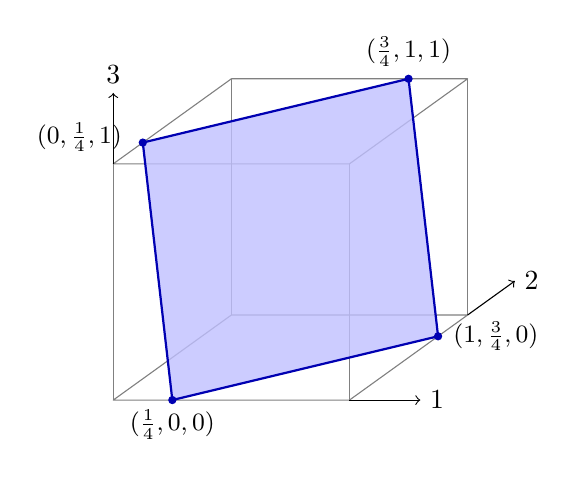
\begin{tikzpicture}[scale=3.0,
  x={(1cm,0cm)}, y={(0.5cm,0.36cm)}, z={(0cm,1cm)}, line join=round]
  % the cube
  \draw[gray] (0,0,0)--(1,0,0)--(1,1,0)--(0,1,0)--cycle;
  \draw[gray] (0,0,1)--(1,0,1)--(1,1,1)--(0,1,1)--cycle;
  \foreach \x/\y in {0/0,1/0,1/1,0/1} \draw[gray] (\x,\y,0)--(\x,\y,1);
  \draw[->] (1,0,0)--(1.3,0,0) node[right] {$1$};
  \draw[->] (1,1,0)--(1,1.4,0) node[right] {$2$};
  \draw[->] (0,0,1)--(0,0,1.3) node[above] {$3$};
  % the square
  \fill[blue!25,opacity=0.8] (0.25,0,0)--(0,0.25,1)--(0.75,1,1)--(1,0.75,0)--cycle;
  \draw[blue!70!black,thick] (0.25,0,0)--(0,0.25,1)--(0.75,1,1)--(1,0.75,0)--cycle;
  \foreach \P in {(0.25,0,0),(0,0.25,1),(0.75,1,1),(1,0.75,0)} \fill[blue!70!black] \P circle (0.5pt);
  \node[below] at (0.25,0,0) {\small $(\frac14,0,0)$};
  \node[left,xshift=-4pt,yshift=2pt] at (0,0.25,1) {\small $(0,\frac14,1)$};
  \node[above,yshift=1pt] at (0.75,1,1) {\small $(\frac34,1,1)$};
  \node[right,xshift=2pt] at (1,0.75,0) {\small $(1,\frac34,0)$};
\end{tikzpicture}
\hspace{1.2cm}
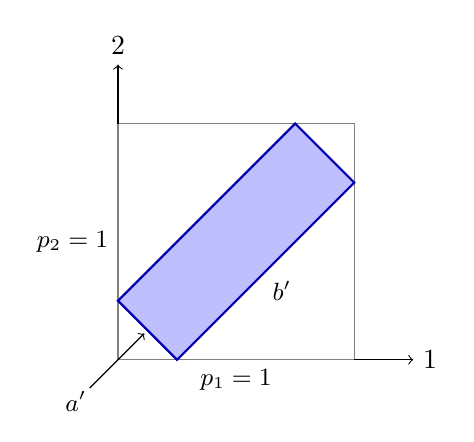
\begin{tikzpicture}[scale=3.0]
  \draw[gray] (0,0) rectangle (1,1);
  \draw[->] (1,0)--(1.25,0) node[right] {$1$};
  \draw[->] (0,1)--(0,1.25) node[above] {$2$};
  \fill[blue!25] (0.25,0)--(1,0.75)--(0.75,1)--(0,0.25)--cycle;
  \draw[blue!70!black,thick] (0.25,0)--(1,0.75)--(0.75,1)--(0,0.25)--cycle;
  \node[below right,xshift=-1pt] at (0.625,0.375) {\small $b'$};
  \draw[->,shorten >=1pt] (-0.12,-0.12) node[below left,inner sep=1pt] {\small $a'$}--(0.12,0.12);
  \node[below] at (0.5,0) {\small $p_1=1$};
  \node[left] at (0,0.5) {\small $p_2=1$};
\end{tikzpicture}
\caption{Left: the largest square $A=B=3\sqrt2/4$ in the unit cube, in the position constructed in
Section~\ref{sec:suff} for $(k,l)=(1,2)$, $S=\{3\}$, $T=\varnothing$. Right: its projection to the plane
of the axes $1,2$ is the $a'\times b'$ rectangle, $a'=\sqrt{A^2-1}=\sqrt2/4$, placed at $45^\circ$ by
Carver's criterion; the rest of the side $A$ goes along the axis $3$.}
\label{fig:example}
\end{figure}

\section{Sufficiency}\label{sec:suff}

Assume (II). Carver's criterion gives orthonormal $f_a,f_b\in\operatorname{span}(e_k,e_l)$ with
$a'\abs{(f_a)_i}+b'\abs{(f_b)_i}\le p_i$ for $i\in\{k,l\}$. Let $\lambda=\min(1,A/\norm{p_S})$ and $\mu=\min(1,B/\norm{p_T})$ (with $\lambda=0$ if $\norm{p_S}=0$ and $\mu=0$ if $\norm{p_T}=0$), $p_S=\sum_{i\in S}p_ie_i$, and
\[
A\,u=\lambda\,p_S+a'f_a,\qquad B\,v=\mu\,p_T+b'f_b .
\]
\begin{itemize}
\item Norms: $\norm{Au}^2=\lambda^2\norm{p_S}^2+a'^2=A^2$ both for $A\ge\norm{p_S}$ and for
$A<\norm{p_S}$ (then $a'=0$). Similarly $\norm{Bv}=B$.
\item Orthogonality: the supports $S$, $T$ and $\{k,l\}$ are pairwise disjoint and $f_a\perp f_b$,
so $u\perp v$.
\item Widths: on $S$ we have $A\abs{u_i}=\lambda p_i\le p_i$ and $v_i=0$; on $T$ symmetrically; on
$\{k,l\}$ by Carver's criterion.
\end{itemize}
By Section~\ref{sec:widths} this is a position of the rectangle in the box. (If $A=0$ put $u=f_a$, and if
$B=0$ put $v=f_b$.) \qed

\section{Reformulation}\label{sec:reform}

\subsection{Reduction to widths}\label{sec:widths}
A box is the intersection of the slabs $\{0\le x_i\le p_i\}$, and shifts along different coordinates are
independent. Hence a convex body can be translated into $P$ if and only if its width along every $e_i$
is at most $p_i$. The width of the rectangle $(Au,Bv)$ along $e_i$ is $A\abs{u_i}+B\abs{v_i}$. Thus
\begin{equation}\label{eq:widths}
\text{the rectangle fits}\iff\exists\ \text{orthonormal } u,v:\quad A\abs{u_i}+B\abs{v_i}\le p_i\ \ \text{for all } i .
\end{equation}

The case $B=0$ (a segment): it fits if and only if $A\le\norm{p}$; the necessity follows from
$A^2=\sum A^2u_i^2\le\sum p_i^2$. This is (I) with $S=[n]$, $T=\varnothing$. From now on $A,B>0$.
Axes with $p_i=0$ are discarded at once: on them $u_i=v_i=0$. If $S,T,k,l$ satisfying (I) or (II) are
found for the remaining axes, each discarded axis is added to $S$; this only increases $\norm{p_S}$,
hence decreases $a'$ and keeps Carver's condition, and it keeps $A\le\norm{p_S}$ in (I).

If fewer than two axes have $p_i>0$, then for $A,B>0$ the rectangle does not fit (two orthonormal
vectors cannot be placed into one coordinate), and (II) is false as well. Indeed, let $m$ be the only
axis with $p_m>0$ (or there is none). If $m\in\{k,l\}$, then $a'=A>0$ and $b'=B>0$, while the box
$(p_m,0)$ holds only a segment; if $m\in S$, then $b'=B>0$ and the box $(0,0)$ is a point; if $m\in T$
(or there is no $m$), then $a'=A>0$ and again the box is a point. So the theorem holds in this case too.

\subsection{Relaxation}\label{sec:relax}
In \eqref{eq:widths} one may require only $\norm u\ge1$, $\norm v\ge1$, $\langle u,v\rangle=0$:
shrinking $u$ or $v$ by a factor $\le1$ keeps the orthogonality and the inequalities. Write
$P_i=p_i^2$, $\alpha_i=A\abs{u_i}/p_i$, $\beta_i=B\abs{v_i}/p_i$ ($\alpha_i+\beta_i\le1$) and
$\sigma_i=\sgn(u_iv_i)\in\{\pm1\}$ (any sign if $u_iv_i=0$). The conditions read
\[
\sum P_i\alpha_i^2\ge A^2,\qquad \sum P_i\beta_i^2\ge B^2,\qquad \sum\sigma_iP_i\alpha_i\beta_i=0 .
\]

\subsection{Active axes}\label{sec:active}
Let $\rho_i=\alpha_i+\beta_i\in[0,1]$ and $p'_i=\rho_ip_i=A\abs{u_i}+B\abs{v_i}\le p_i$. In the box $p'$
with the same $u,v$ every axis is \emph{active}: $\alpha'_i+\beta'_i=1$. Put
$\alpha'_i=(1+t_i)/2$, $\beta'_i=(1-t_i)/2$, $t_i\in[-1,1]$. The conditions of Section~\ref{sec:relax}
for $p'$ are the same, since $P'_i\alpha'^2_i=A^2u_i^2$ and so on. Axes with $\rho_i=0$ are discarded.

Conditions (I) and (II) are monotone in $p$: when $p$ grows, the norms $\norm{p_S}$ grow, so $a'$, $b'$ do
not grow, while the box $(p_k,p_l)$ grows. Hence (I)$\vee$(II) for $p'$ implies (I)$\vee$(II) for $p$.
\emph{Therefore it suffices to prove that an active configuration in the box $p$ satisfies (I) or (II).}
From now on we keep the notation $p$ for the box in which all axes are active.

An active configuration is a pair $(t,\sigma)$, $t\in[-1,1]^n$, $\sigma\in\{\pm1\}^n$, with
$A\abs{u_i}=p_i(1+t_i)/2$, $B\abs{v_i}=p_i(1-t_i)/2$ and $\sgn(u_iv_i)=\sigma_i$. The \emph{sides} are
$+=\{i:\sigma_i=+1\}$ and $-=\{i:\sigma_i=-1\}$. An axis is \emph{mixed} if $\abs{t_i}<1$, that is, $u_iv_i\ne0$.

Conversely, let all $p_i>0$ and let $(t,\sigma)$ be any pair. Put $\abs{u_i}=p_i(1+t_i)/(2A)$,
$\abs{v_i}=p_i(1-t_i)/(2B)$ and choose the signs so that $\sgn(u_iv_i)=\sigma_i$ whenever $u_iv_i\ne0$.
Then all widths equal $p_i$, and
\[
\norm u^2=\sum\frac{P_i(1+t_i)^2}{4A^2},\qquad \norm v^2=\sum\frac{P_i(1-t_i)^2}{4B^2},\qquad
\langle u,v\rangle=\sum\frac{\sigma_iP_i(1-t_i^2)}{4AB}.
\]
We call $(t,\sigma)$ \emph{admissible} if $\norm u\ge1$, $\norm v\ge1$ and $\langle u,v\rangle=0$. By
Section~\ref{sec:relax} an admissible configuration gives a position of the rectangle. All configurations
built in Section~\ref{sec:lemmas} are given by pairs $(t',\sigma')$, and their admissibility is checked
through these three conditions only; an equivalent form of them follows.

\subsection{The tent}\label{sec:tent}
Let $L=\sum P_it_i$, $\Def_\pm=\sum_{i\in\pm}P_i(1-t_i^2)$, $W=\sum P_i$, $c_A=2A^2-W$, $c_B=W-2B^2$.
\begin{itemize}
\item Orthogonality $\sum\sigma_iP_i(1-t_i^2)=0$ means $\Def_+=\Def_-=:D$.
\item Then $\sum P_it_i^2=W-2D$, and
$\sum P_i(1+t_i)^2\ge4A^2\iff L-D\ge c_A$, $\ \sum P_i(1-t_i)^2\ge4B^2\iff L+D\le c_B$.
\end{itemize}
So a configuration with $\Def_+=\Def_-=D$ is admissible if and only if the point $(L,D)$ lies under the
``tent'' $\{D\le L-c_A,\ D\le c_B-L\}$ (Figure~\ref{fig:tent}). The tent is $1$-Lipschitz, hence:

\medskip\noindent$(\star)$ \emph{If $(t,\sigma)$ is admissible and $(t',\sigma')$ is another configuration
with $\Def'_+=\Def'_-=D'$ and $D'+\abs{L'-L}\le D$, then $(t',\sigma')$ is admissible.}
Indeed, $L'-D'\ge L'-D+\abs{L'-L}\ge L-D\ge c_A$ and $L'+D'\le L+D\le c_B$.

\medskip
A mixed axis contributes a positive amount to $\Def$ of its side. Since $\Def_+=\Def_-$, mixed axes
are either present on both sides or absent altogether; exactly one mixed axis is impossible.

\begin{figure}[ht]
\centering
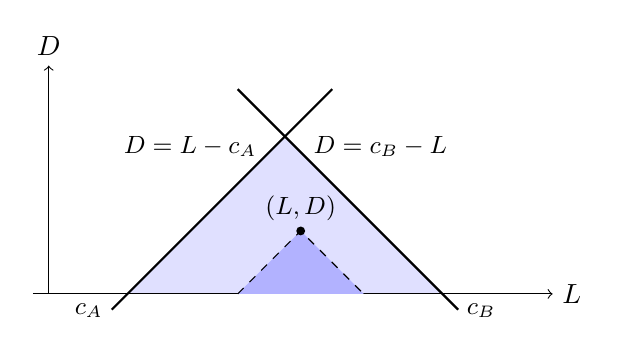
\begin{tikzpicture}[scale=1.0]
  \fill[blue!12] (-1,0)--(1,2)--(3,0)--cycle;
  \draw[->] (-2.2,0)--(4.4,0) node[right] {$L$};
  \draw[->] (-2,0)--(-2,2.9) node[above] {$D$};
  \draw[thick] (-1.2,-0.2)--(1.6,2.6) node[pos=0.74,left,xshift=-3pt] {\small $D=L-c_A$};
  \draw[thick] (0.4,2.6)--(3.2,-0.2) node[pos=0.26,right,xshift=3pt] {\small $D=c_B-L$};
  \node[below,xshift=-14pt] at (-1,0) {\small $c_A$};
  \node[below,xshift=14pt] at (3,0) {\small $c_B$};
  \fill[blue!30] (1.2,0.8)--(0.4,0)--(2.0,0)--cycle;
  \draw[dashed] (0.4,0)--(1.2,0.8)--(2.0,0);
  \fill (1.2,0.8) circle (1.6pt) node[above] {\small $(L,D)$};
\end{tikzpicture}
\caption{Admissible configurations correspond to points $(L,D)$ under the tent. Every point
$(L',D')$ with $D'+\abs{L'-L}\le D$ (the darker triangle below $(L,D)$) is again under the tent; this is $(\star)$.}
\label{fig:tent}
\end{figure}

\section{Three lemmas}\label{sec:lemmas}

\begin{lemma}[C: at most two mixed axes]\label{lem:C}
If an admissible configuration has no mixed axes, then (I) holds. If it has exactly two mixed axes,
$k\in+$ and $l\in-$, then (II) holds with these $k,l$.
\end{lemma}
\begin{proof}
No mixed axes. Put $S=\{t=+1\}$, $T=\{t=-1\}$. Then $D=0$, $L=\norm{p_S}^2-\norm{p_T}^2$,
$W=\norm{p_S}^2+\norm{p_T}^2$, and the tent gives $\norm{p_S}^2\ge A^2$, $\norm{p_T}^2\ge B^2$; this is (I).

Two mixed axes $k\in+$, $l\in-$. On the other axes $u_iv_i=0$, so for $U=(u_k,u_l)$, $V=(v_k,v_l)$ we have
$\langle U,V\rangle=\langle u,v\rangle=0$; also $U,V\ne0$ because $u_iv_i\ne0$ on a mixed axis. Hence the
rectangle $A\abs U\times B\abs V$ with directions $U/\abs U$, $V/\abs V$ lies in the $2$-box
$(p_k,p_l)$: its widths are $A\abs{u_i}+B\abs{v_i}=p_i$. Let $S=\{t=+1\}$; there $v_i=0$ and
$A\abs{u_i}=p_i$. Then $A^2\abs U^2=A^2\norm u^2-\norm{p_S}^2\ge A^2-\norm{p_S}^2$ (the axes with
$t=-1$ do not contribute to $u$), that is, $A\abs U\ge a'$. Similarly $B\abs V\ge b'$ for $T=\{t=-1\}$. By
monotonicity $\Carver(a',b';p_k,p_l)$ holds; this is (II).
\end{proof}

\begin{lemma}[R: opposite signs]\label{lem:R}
Suppose all mixed axes of the side $+$ have $t\ge0$ and all mixed axes of the side $-$ have $t\le0$ (or
the other way round). Then (I) holds.
\end{lemma}
\begin{proof}
Round: $t\mapsto+1$ on the mixed axes of the side $+$ and $t\mapsto-1$ on the mixed axes of the side $-$.
\begin{itemize}
\item The shift of $L$ from the side $+$ is $\Delta_+=\sum P(1-t)\in[0,D]$, since $1-t\le1-t^2$ for $t\in[0,1]$.
\item The shift of $L$ from the side $-$ is $\Delta_-=-\sum P(1+t)\in[-D,0]$, since $1+t\le1-t^2$ for $t\in[-1,0]$.
\item In the new configuration $\Def'_+=\Def'_-=0$ and $\abs{L'-L}=\abs{\Delta_++\Delta_-}\le D$, the
summands having opposite signs.
\end{itemize}
By $(\star)$ it is admissible. It has no mixed axes, so Lemma~\ref{lem:C} gives (I). The other case is symmetric.
\end{proof}

\begin{lemma}[V: moving along a curve]\label{lem:V}
Let $i\ne j$ be mixed axes of one side (say $+$) and $k$ a mixed axis of the other side, $s_0=t_k$.
Suppose that it is not the case that $t_i=t_j$ and $t_is_0\le0$; that is, either (a) $t_i\ne t_j$, or
(b) $t_i=t_j$ and $t_is_0>0$. Then there is an admissible configuration with a smaller $D$.
\end{lemma}
\begin{proof}
We change only $(t_i,t_j,t_k)$, keeping $L$ and $\Def_+-\Def_-$:
\[
P_it_i+P_jt_j=\lambda(s):=L_0-P_ks,\qquad P_it_i^2+P_jt_j^2=\mu(s):=K_0+P_ks^2,\qquad t_k=s .
\]
Then $D=\Def_-=\mathrm{const}+P_k(1-s^2)$ strictly decreases as $\abs s$ grows, while $L$ does not change.
By $(\star)$ the configuration stays admissible as long as $(t_i,t_j,t_k)\in[-1,1]^3$. (The other mixed axes
of the side $+$, if any, enter the constants $L_0$, $K_0$.)

The line $\{P_iX+P_jY=\lambda\}$ and the ellipse $\{P_iX^2+P_jY^2=\mu\}$ intersect if and only if
$h(s):=\mu(s)-\lambda(s)^2/(P_i+P_j)\ge0$: by the Cauchy--Schwarz inequality the minimum of
$P_iX^2+P_jY^2$ on the line is attained at $X=Y=\tau:=\lambda/(P_i+P_j)$, and $h=0$ means tangency,
$t_i=t_j=\tau$. We have $h'(s)=2P_k(s+\tau)$.

(a) If $t_i\ne t_j$, the Jacobian of $(X,Y)\mapsto(P_iX+P_jY,\,P_iX^2+P_jY^2)$ equals
$2P_iP_j(Y-X)\ne0$, and by the implicit function theorem the solution extends to $s$ close to $s_0$, in
particular to $\abs s>\abs{s_0}$ (for $s_0=0$ in either direction). The point $(t_i,t_j)$ is inside the
square $(-1,1)^2$ and $\abs{s_0}<1$, so for a small move everything stays in $[-1,1]$, and $D$ strictly decreases.

(b) If $t_i=t_j=\tau$ and $\tau s_0>0$, then $s_0\ne0$, $h(s_0)=0$, and $h'(s_0)=2P_k(s_0+\tau)$ has the sign
of $s_0$. Hence $h>0$ for a small increase of $\abs s$, and there are two intersection points. Since $i,j$ are
mixed, $\abs\tau<1$; choose $\varepsilon>0$ with $\abs\tau+2\varepsilon<1$. Both intersection points depend
continuously on $s$ and tend to $(\tau,\tau)$ as $s\to s_0$ (the distance to the tangency point is of order
$\sqrt h$). So for a small enough change of $s$ both coordinates stay in $(-\abs\tau-\varepsilon,\abs\tau+\varepsilon)\subset(-1,1)$,
and also $\abs s<1$. Again $D$ strictly decreases.
\end{proof}

\section{Necessity}\label{sec:nec}

By Section~\ref{sec:reform} it suffices to consider an admissible active configuration in the box $p$ with all
$p_i>0$. For each of the finitely many $\sigma$ the set of admissible $t\in[-1,1]^n$ is given by the closed
conditions $\Def_+=\Def_-$, $L-D\ge c_A$, $L+D\le c_B$, where $L$, $\Def_\pm$ and $D$ are polynomials in $t$;
so it is compact. For the $\sigma$ of the given configuration it is nonempty, and $D\ge0$ is continuous, so there is a configuration with the
\emph{smallest} $D$.
\begin{enumerate}
\item If some side has two mixed axes with different $t$, then the other side has a mixed axis too
(Section~\ref{sec:tent}), and Lemma~\ref{lem:V}(a) decreases $D$, a contradiction. So all mixed axes of the
side $+$ have a common $t=\tau$, and all mixed axes of the side $-$ a common $t=s$.
\item If each side has at most one mixed axis, then by Section~\ref{sec:tent} there are $0$ or $1+1$ of them,
and Lemma~\ref{lem:C} applies.
\item Otherwise some side (say $+$) has at least two mixed axes with the common $\tau$. Take a mixed axis $k$ of
the other side, $t_k=s$. If $\tau s>0$, Lemma~\ref{lem:V}(b) decreases $D$, a contradiction. So $\tau s\le0$,
the sign conditions of Lemma~\ref{lem:R} hold, and we get (I). \qed
\end{enumerate}

\begin{corollary}\label{cor:structure}
Suppose (I) fails. Then every admissible configuration with the smallest $D$ has exactly two mixed axes, one on each
side, and their $t$ have the same sign. In other words, an optimal position has the form (II) with a rotation in a
single coordinate plane.
\end{corollary}
\begin{proof}
No mixed axes would give (I) by Lemma~\ref{lem:C}; two or more on one side lead by items 1 and 3 to a contradiction
or to (I); opposite signs would give (I) by Lemma~\ref{lem:R}.
\end{proof}

\section{(I) is a special case of (II)}\label{sec:I}

Let $A,B>0$ and (I) hold. Then $S$ and $T$ are nonempty, since $\norm{p_S}\ge A>0$ and $\norm{p_T}\ge B>0$.
Let $R=[n]\setminus(S\cup T)$, take $k\in S$, $l\in T$ and put $S'=(S\setminus\{k\})\cup R$, $T'=T\setminus\{l\}$,
so that $S'\sqcup T'=[n]\setminus\{k,l\}$. Then $\norm{p_{S'}}^2=\norm{p_S}^2-p_k^2+\norm{p_R}^2\ge A^2-p_k^2$,
whence $a'^2\le p_k^2$; similarly $b'^2\le p_l^2$, and Carver's condition holds without rotation. For $B=0$ take any
$k\ne l$, $S=$ the other axes, $T=\varnothing$: the segment $a'$ fits into $(p_k,p_l)$ if and only if
$a'\le\sqrt{p_k^2+p_l^2}$, that is, $A\le\norm p$.

Together with Sections~\ref{sec:suff}--\ref{sec:nec} this proves Theorem~\ref{thm:main}. As by-products:
\eqref{eq:widths} has a solution with at most two coordinates where $u_iv_i\ne0$; and if (I) fails, the two mixed
axes in (II) have $t$ of the same sign.

\section{The unit cube: Theorem~5 of Jerrard and Wetzel}\label{sec:jw}

Jerrard and Wetzel \cite[Theorem~5, formula~(8)]{JerrardWetzel2004} found the largest $L\times\lambda L$
rectangle, $0\le\lambda\le1$, in the unit cube:
$L_{\max}=f_1(\lambda)$ on $[0,\lambda_1]$, $\sqrt2$ on $[\lambda_1,\lambda_2]$ and $f_3(\lambda)$ on $[\lambda_2,1]$, where
\[
f_1(\lambda)=\frac{3}{\sqrt{3-\lambda^2}+\sqrt2\lambda},\qquad f_3(\lambda)=\frac{3}{\sqrt2+\sqrt{3\lambda^2-1}},\qquad
\lambda_1=1-\tfrac{\sqrt2}{2},\quad \lambda_2=\tfrac{\sqrt2}{2}.
\]
Theorem~\ref{thm:main} gives the same answer by a different route. Let $p=(1,1,1)$, $A=L$, $B=\lambda L$, and let $m$
be the third axis, $\{k,l,m\}=\{1,2,3\}$.
\begin{itemize}
\item $m\in S$, $A>1$: $a'=\sqrt{A^2-1}$, $b'=\lambda A$, and Carver in the unit square gives
$\sqrt{A^2-1}+\lambda A\le\sqrt2$, that is, $(1-\lambda^2)A^2+2\sqrt2\lambda A-3\le0$, or $A\le f_1(\lambda)$.
\item $m\in T$, $B\le1$: $b'=0$, a segment $A$ in the unit square, $A\le\sqrt2$; here $B=\lambda\sqrt2\le1$ means $\lambda\le\sqrt2/2$.
\item $m\in T$, $B>1$: $a'=A$, $b'=\sqrt{\lambda^2A^2-1}$, and Carver gives $A+\sqrt{\lambda^2A^2-1}\le\sqrt2$, that is,
$A\le f_3(\lambda)$. This is feasible only for $\lambda\ge\lambda_2$: the left-hand side grows in $A$ and equals
$1/\lambda$ at $A=1/\lambda$, so $1/\lambda\le\sqrt2$ is needed.
\item The rectangle without rotation gives $\min(\sqrt2,1/\lambda)$, which is never better.
\end{itemize}
The denominators of $f_1$ and $f_3$ increase in $\lambda$, so $f_1$ and $f_3$ decrease, and $f_1(\lambda_1)=f_3(\lambda_2)=\sqrt2$.
On $[\lambda_2,1]$ we have $f_3\ge f_1$: the difference of the denominators
$\varphi=(\sqrt{3-\lambda^2}+\sqrt2\lambda)-(\sqrt2+\sqrt{3\lambda^2-1})$ vanishes at $\lambda=1$ and decreases, since
$\varphi'\le\sqrt2-3\lambda/\sqrt{3\lambda^2-1}\le\sqrt2-3/\sqrt2<0$. So the maximum over these variants is exactly
$L_{\max}(\lambda)$. Jerrard and Wetzel argue by the positions of the vertices; here the variants are partitions of
the axes. Numerically, the enumeration of all $(k,l,S,T)$ with bisection agrees with formula~(8) on $1001$ values of
$\lambda\in[0,1]$ up to $3.3\cdot10^{-16}$.

\section{The formal proof}\label{sec:lean}

The theorem has been proved in Lean~4 with Mathlib; the sources are in the directory \texttt{lean/} of the
repository \cite{Repo}. The meaning of the main theorem depends only on the following definitions
(file \texttt{Widths.lean}):
\begin{verbatim}
abbrev En (n : ℕ) := EuclideanSpace ℝ (Fin n)
def boxN (q : Fin n → ℝ) : Set (En n) := {x | ∀ i, 0 ≤ x i ∧ x i ≤ q i}
noncomputable def pad (h : m ≤ n) (q : Fin m → ℝ) : Fin n → ℝ :=
  Function.extend (Fin.castLE h) q 0
def FitsN (p q : Fin n → ℝ) : Prop := ∃ f : En n ≃ᵢ En n, f '' boxN q ⊆ boxN p
\end{verbatim}
Here \texttt{pad h ![A, B]} is the vector of edges $(A,B,0,\dots,0)$, so the rectangle is the box
\texttt{boxN (pad h ![A, B])} in $\R^n$, and \texttt{FitsN} asks for an isometry of $\R^n$ (any rigid motion,
reflections included) mapping one box into the other. Carver's criterion is written verbatim as in
Section~\ref{sec:thm} (\texttt{CarverS} for sorted sides, \texttt{Carver} sorts by \texttt{max}/\texttt{min}).
The main theorem (file \texttt{RectCarver.lean}) reads
\begin{verbatim}
theorem fitsN_rect_iff_explicit (h : 2 ≤ n) (p : Fin n → ℝ) (hp : ∀ i, 0 ≤ p i)
    {A B : ℝ} (hA : 0 ≤ A) (hB : 0 ≤ B) :
    FitsN p (pad h ![A, B]) ↔
      ∃ k l : Fin n, k ≠ l ∧ ∃ S T : Finset (Fin n), Disjoint S T ∧
        S ∪ T = univ \ {k, l} ∧
        Carver (√(A ^ 2 - ∑ i ∈ S, p i ^ 2)) (√(B ^ 2 - ∑ i ∈ T, p i ^ 2))
          (p k) (p l)
\end{verbatim}
(in Mathlib $\sqrt x=0$ for $x\le0$, so the positive part is automatic). The command \texttt{\#print axioms}
reports only the standard axioms \texttt{propext}, \texttt{Classical.choice}, \texttt{Quot.sound}; the
sources contain no \texttt{sorry}. Versions: Lean~4 v4.34.0-rc2, Mathlib v4.34.0-rc2. The hypotheses are only
$n\ge2$, $p_i\ge0$, $A,B\ge0$, so the degenerate cases $A=0$ or $B=0$ (a segment, a point) are covered by the
same statement.

The formalization follows Sections~\ref{sec:suff}--\ref{sec:I} with a few simplifications.
Instead of passing to active axes, it works with $x=Au$, $y=Bv$ and the local widths
$r_i=\abs{x_i}+\abs{y_i}\le p_i$, which all steps preserve; it minimizes $\sum\abs{x_iy_i}$ (which is $D/2$) over
all solutions of the relaxed problem at once, without fixing $\sigma$; and Lemma~\ref{lem:V} is proved without the
implicit function theorem, by the explicit parametrization $X=\tau+P_j\theta$, $Y=\tau-P_i\theta$ of the line, for
which $P_iX^2+P_jY^2=(P_i+P_j)\tau^2+P_iP_j(P_i+P_j)\theta^2$. Carver's criterion itself is proved from the strip
lemma of \cite{Levit2026}: if $a>X$, the optimal position of the $a\times b$ rectangle touches the strip of width $X$,
and it remains to compare its extent along the strip with $Y$, which is pure algebra.

\section{Computation}\label{sec:comp}

The criterion runs through $\tfrac12n(n-1)2^{n-2}$ cases, each a Carver test with two square roots; the
number of cases grows exponentially with $n$, but for $n\le10$ it is at most $11\,520$. Further,
Section~\ref{sec:suff} turns a successful case into an explicit orthonormal pair $(u,v)$. We compared a Python
implementation (\texttt{tools/rect\_fit.py} in \cite{Repo}) with two numerical searches over positions: the
Nelder--Mead method on $F(u,v)=\max_i(A\abs{u_i}+B\abs{v_i})/p_i$ over orthonormal pairs (as in
\cite{Levit2026}), and the SLSQP method on the smooth lifted problem ``minimize $t$ subject to
$A a_i+Bb_i\le tp_i$, $a_i\ge\abs{u_i}$, $b_i\ge\abs{v_i}$, $\norm u=\norm v=1$, $u\perp v$'', both from random starts.
A numerical search answers ``fits'' as soon as some start reaches $F\le1$; it cannot confirm that the rectangle does
not fit. For each $n$ we took $50$ pairs near the boundary: the rectangle is scaled by $t^*(1\pm e)$, where $t^*$ is
the largest scale at which it fits and $10^{-4}\le e\le10^{-2}$; about half of them fit. Timings per pair
(Python~3.10, one core). The criterion stops at the first successful case; the column ``criterion'' is
averaged over all pairs, including those that do not fit and need all cases, while the column
``criterion + position'' is averaged over the fitting pairs only, which is why it can be smaller.

\begin{center}
\begin{tabular}{ccccc}
\toprule
$n$ & criterion & criterion + position & Nelder--Mead, 20 starts & SLSQP, 20 starts\\
\midrule
3 & 6\,$\mu$s & 7\,$\mu$s & 1.0 s; missed 3 of 25 & 26 ms; missed 1 of 25\\
4 & 26\,$\mu$s & 21\,$\mu$s & 1.9 s; missed 19 of 22 & 40 ms; missed 1 of 22\\
5 & 80\,$\mu$s & 36\,$\mu$s & 2.4 s; missed 24 of 24 & 46 ms; missed 2 of 24\\
6 & 194\,$\mu$s & 42\,$\mu$s & 3.3 s; missed 24 of 24 & 63 ms; missed 3 of 24\\
\bottomrule
\end{tabular}
\end{center}

\noindent ``Missed'' means that the search answered ``does not fit'' for a rectangle that fits. No search ever found a
position where the criterion says ``does not fit''. All positions produced by the criterion passed the check (orthonormality and widths), both here and in a
separate self-test of the implementation on $20\,000$ random pairs with $n=2,\dots,7$ (not timed). Floating-point comparisons are
exact only in exact arithmetic: near the boundary rounding may flip the answer.

\section{Remarks}\label{sec:remarks}

The argument uses a single pair of orthogonal columns $(u,v)$, that is, a single orthogonality condition, which
takes the form $\Def_+=\Def_-$. This is why the problem fits into the two-dimensional picture $(L,D)$ of the tent.
For a box with three nonzero edges there are three such conditions; each pair of the columns gives its own
partition of the axes into sides, and a move of Lemma~\ref{lem:V} preserving one condition breaks the other two.
This is an explanation, not a proof. For a three-dimensional box in a three-dimensional box an explicit criterion
is known \cite{Levit2026}; for $k\ge3$ and $d\ge4$ the problem of Jerrard and Wetzel remains open, as far as we know.

\begin{thebibliography}{99}
\bibitem{Carver1957} W.~B.~Carver, Solution of Problem E1225, \emph{Amer. Math. Monthly} 64 (1957) 114--116.
\bibitem{JerrardWetzel2004} R.~P.~Jerrard, J.~E.~Wetzel, Prince Rupert's rectangles, \emph{Amer. Math. Monthly} 111 (2004) 22--31.
\bibitem{Levit2026} M.~Levit, When does a box fit into a box? An explicit criterion with a formal proof, 2026,
\url{https://github.com/MikhailLevit1987/box-in-box}, \href{https://doi.org/10.5281/zenodo.22974798}{doi:10.5281/zenodo.22974798}.
\bibitem{Repo} M.~Levit, Rectangle in an $n$-dimensional box: paper, Lean formalization and code, 2026,
\url{https://github.com/MikhailLevit1987/rectangle-in-n-box}.
\bibitem{vanSwinden1816} J.~H.~van Swinden, \emph{Grondbeginsels der Meetkunde}, 2nd ed., P.~den Hengst en Zoon, Amsterdam, 1816, pp.~512--513, 608--610.
\bibitem{Wetzel2000} J.~E.~Wetzel, Rectangles in rectangles, \emph{Math. Mag.} 73 (2000) 204--211.
\end{thebibliography}

\end{document}
